% !TeX spellcheck = de_DE
\documentclass[ngerman,12pt]{article}

% Packages for Language
\usepackage[ngerman]{babel}
\usepackage[utf8]{inputenc}
\usepackage[T1]{fontenc}
\usepackage[final]{graphicx}
\usepackage{amsmath}
\usepackage{float}
%\usepackage{wrapfig}
\usepackage{caption}
%\usepackage{multirow}
\usepackage{subfig}
\usepackage{hyperref}
\usepackage[german, plain]{fancyref}
\usepackage{afterpage,pdflscape} %%% !!!!!!! CHANGE TO PDFLSCAPE LATER!
\usepackage{varioref}
\usepackage{siunitx}
\usepackage{translator}
\usepackage{listings}
\usepackage{fancyhdr}
\pagestyle{fancy}

\setlength{\headheight}{15.5pt}
\lhead{NAME NAME NAME}
\rhead{\today}
\chead{Numerik Übung 5}


\begin{document}
\lstset{language=Matlab,basicstyle=\ttfamily,columns=fixed}
\subsubsection*{strassen.m}
\begin{lstlisting}[frame=single]
function [ C ] = strassen( A, B )
[~,n] = size(A);
if n == 1
  C = A*B;
else
  un = 1:(n/2);
  ln = (n/2)+1:n;
  
  A11 = A(un,un);
  A12 = A(un,ln);
  A21 = A(ln,un);
  A22 = A(ln,ln);
  B11 = B(un,un);
  B12 = B(un,ln);
  B21 = B(ln,un);
  B22 = B(ln,ln);
  
  P1 = strassen((A11+A22), (B11+B22));
  P2 = strassen((A21+A22), B11);
  P3 = strassen(A11, (B12-B22));
  P4 = strassen(A22, (B21-B11));
  P5 = strassen((A11+A12), B22);
  P6 = strassen((A21-A11), (B11+B12));
  P7 = strassen((A12-A22), (B21+B22));
  
  C = [(P1+P4-P5+P7),(P3+P5);(P2+P4),(P1+P3-P2+P6)];
end
end
\end{lstlisting}
\filbreak

\subsubsection*{A5}
\begin{lstlisting}[frame=single]
ns = 2.^(3:9); ts = zeros(size(ns));
for ii=1:length(ns)
disp(['n = ' num2str(ns(ii))]);
A = rand(ns(ii)); B = rand(ns(ii));
tic; C = strassen(A, B); ts(ii) = toc;
disp(['Error is ' num2str(norm(C-A*B, 'fro')) '.']);
end
loglog(ns, ts, 'r-s', ns, ts(2)*(ns(2)\ns).^3, ...
'b-.', ns, ts(2)*(ns(2)\ns).^log2(7), 'k--');
legend('Laufzeit', 'n^3', 'n^{log_2(7)}', ...
 'Location', 'NorthWest');
\end{lstlisting}

\subsubsection*{Output}
\begin{lstlisting}[frame=single]
>> main
n = 8
Error is 1.163e-14.
n = 16
Error is 6.4715e-14.
n = 32
Error is 3.8185e-13.
n = 64
Error is 3.5229e-12.
n = 128
Error is 2.0668e-11.
n = 256
Error is 1.5744e-10.
n = 512
Error is 1.1109e-09.
\end{lstlisting}

\begin{figure}[h]
    \centering
    
    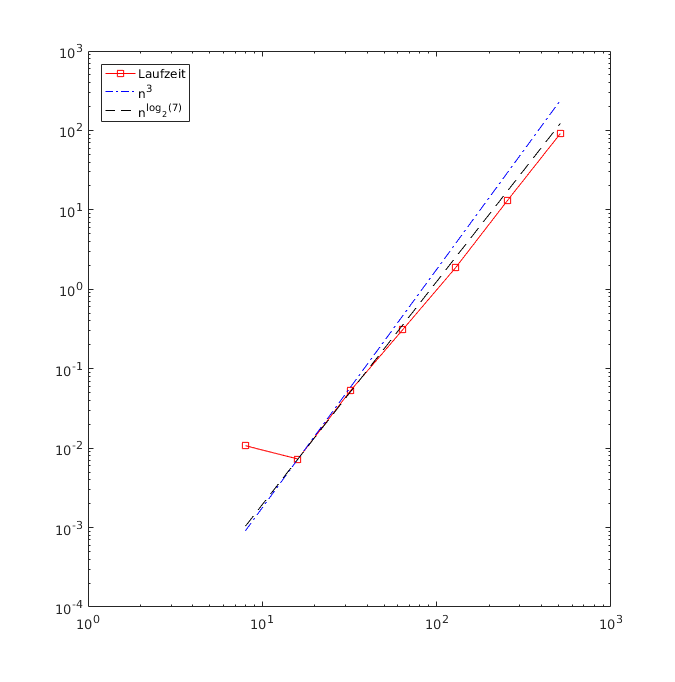
\includegraphics[width=\columnwidth]{A5v.png}
    \caption{Ergebnis}
    \label{fig:ergebnis}
\end{figure}

\end{document}